% !TeX spellcheck = en_US

%TODO Leena

\begin{frame}{9-Intersection}
	\begin{block}{Goal} 
	A computational model to describe conceptual neighborhoods and enable the definition of a similarity metric for line region relations.
		\end{block}
	\begin{block}{Conceptual Similarity: Which pairs of relationships are similar?}
	\begin{figure}
	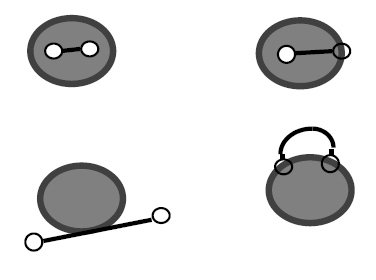
\includegraphics[width = 0.5\textwidth]{images/conceptualsimilarity.png}
	\end{figure}
\end{block}			
\end{frame}

\begin{frame}{Formal Definitions}
	\begin{block}{Line}
	A sequence of 1...n connected 1-cells between two geometrically independent 0-cells such that they neither cross each other nor form cycles.
	\begin{itemize}
	\item Interior, Boundary, Exterior
	\end{itemize}
\end{block}		
		\begin{figure}
		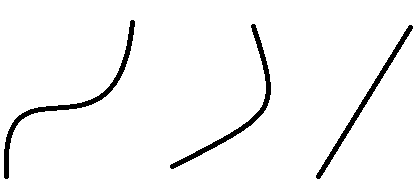
\includegraphics[width=0.7\textwidth]{images/line.png}
\end{figure}
\end{frame}

\begin{frame}{Formal Definitions(contd.,)}
	\begin{block}{Region}
	A region is defined as a connected, homogeneously 2-dimensional 2-cell. Its boundary forms a Jordan curve separating the region's exterior from its interior.
	\begin{itemize}
	\item Interior, Boundary, Exterior
	\end{itemize}
\end{block}		
		\begin{figure}
		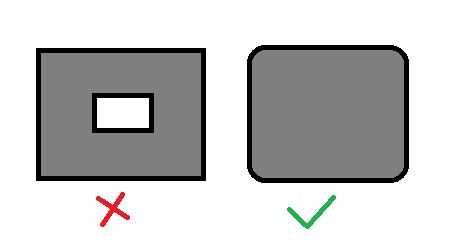
\includegraphics[width=0.7\textwidth]{images/region.png}
\end{figure}
\end{frame}

\begin{frame}{Adjacency}
	\begin{block}{Topological adjacency}
	\begin{itemize}
	\item Adjacent(Interior {$A^0$}) = $\partial A$
	\item Adjacent(Boundary {$\partial A$}) = $A^0 and A^-$
	\item Adjacent(Exterior {$A^-$}) = $\partial A$
	\end{itemize}
	\begin{figure}
	
\includegraphics[width = 0.5\textwidth]{images/adjacency.png}
	\end{figure}
\end{block}		
\end{frame}

\begin{frame}{Adjacency}
	\begin{block}{Topological adjacency}
	\begin{itemize}
	\item Adjacent(Interior {$A^0$}) = $\partial A$
	\item Adjacent(Boundary {$\partial A$}) = $A^0 and A^-$
	\item Adjacent(Exterior {$A^-$}) = $\partial A$
	\end{itemize}
	\begin{figure}
	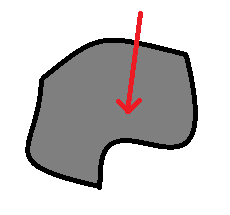
\includegraphics[width = 0.5\textwidth]{images/interior.png}
	\end{figure}
\end{block}		
\end{frame}

\begin{frame}{Adjacency}
	\begin{block}{Topological adjacency}
	\begin{itemize}
	\item Adjacent(Interior {$A^0$}) = $\partial A$
	\item Adjacent(Boundary {$\partial A$}) = $A^0 and A^-$
	\item Adjacent(Exterior {$A^-$}) = $\partial A$
	\end{itemize}
	\begin{figure}
	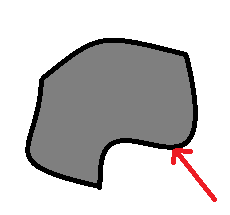
\includegraphics[width = 0.5\textwidth]{images/boundary.png}
	\end{figure}
\end{block}		
\end{frame}

\begin{frame}{Adjacency}
	\begin{block}{Topological adjacency}
	\begin{itemize}
	\item Adjacent(Interior {$A^0$}) = $\partial A$
	\item Adjacent(Boundary {$\partial A$}) = $A^0 and A^-$
	\item Adjacent(Exterior {$A^-$}) = $\partial A$
	\end{itemize}
	\begin{figure}
	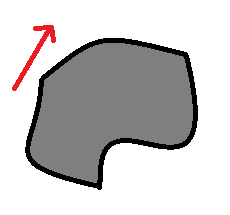
\includegraphics[width = 0.5\textwidth]{images/exterior.png}
	\end{figure}
\end{block}		
\end{frame}

\begin{frame}{9-Intersection(contd..,)}
	\begin{block}{Topological adjacency}
	\begin{itemize}
	\item 9 intersections between the different topological parts of a line and a region
	\end{itemize}
\end{block}		
\begin{block}{The 9-intersection Matrix(M)}
\[ \left( \begin{array}{ccc}
L^0 \cap R^0  & L^0 \cap \partial R & L^0 \cap R^- \\
\partial L \cap R^0 & \partial L \cap \partial R & \partial L \cap R^- \\
L^- \cap R^0 & L^- \cap \partial R & L^- \cap R^- \end{array} \right)\] 
\end{block}
\end{frame}

\begin{frame}{9-Intersection(contd..,)}
	\begin{block}{}
	\begin{itemize}
	\item Binary assignment to intersections($\emptyset,  -\emptyset$)
	\item \textbf{512} possible instances of M
	\item \textbf{19} of 512 instances can actually be realized.
	\end{itemize}
\end{block}		
\begin{block}{Example}
\begin{figure}[l]
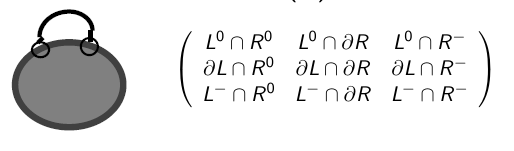
\includegraphics[width = \textwidth]{images/9examplemat.png}
\end{figure} 
\end{block}
\end{frame}

\begin{frame}{9-Intersection(contd..,)}
	\begin{block}{}
	\begin{itemize}
	\item Binary assignment to intersections($\emptyset,  -\emptyset$)
	\item \textbf{512} possible instances of M
	\item \textbf{19} of 512 instances can actually be realized.
	\end{itemize}
\end{block}		
\begin{block}{Example}
\begin{figure}[l]
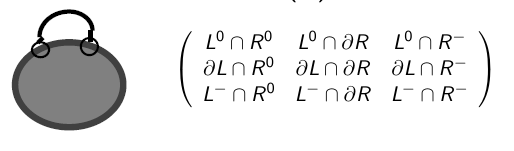
\includegraphics[width = \textwidth]{images/9examplemat.png}
\end{figure} 
Compute the values of the matrix...
\end{block}
\end{frame}


\begin{frame}{Geometric interpretations}	
\begin{figure}[l]
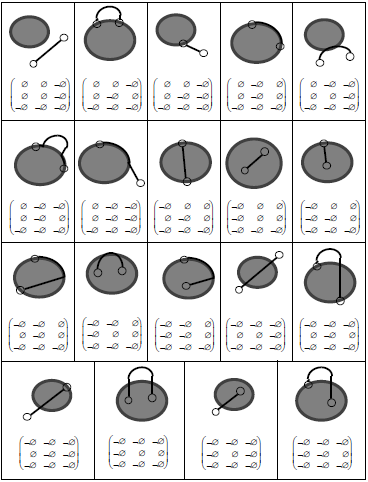
\includegraphics[width = 0.55\textwidth]{images/9intersection.png}
\end{figure} 
\end{frame}

